\documentclass[varwidth=true, border=2pt]{standalone}

\usepackage{tkz-fct}
\usetikzlibrary{arrows, decorations.pathreplacing}

\begin{document}
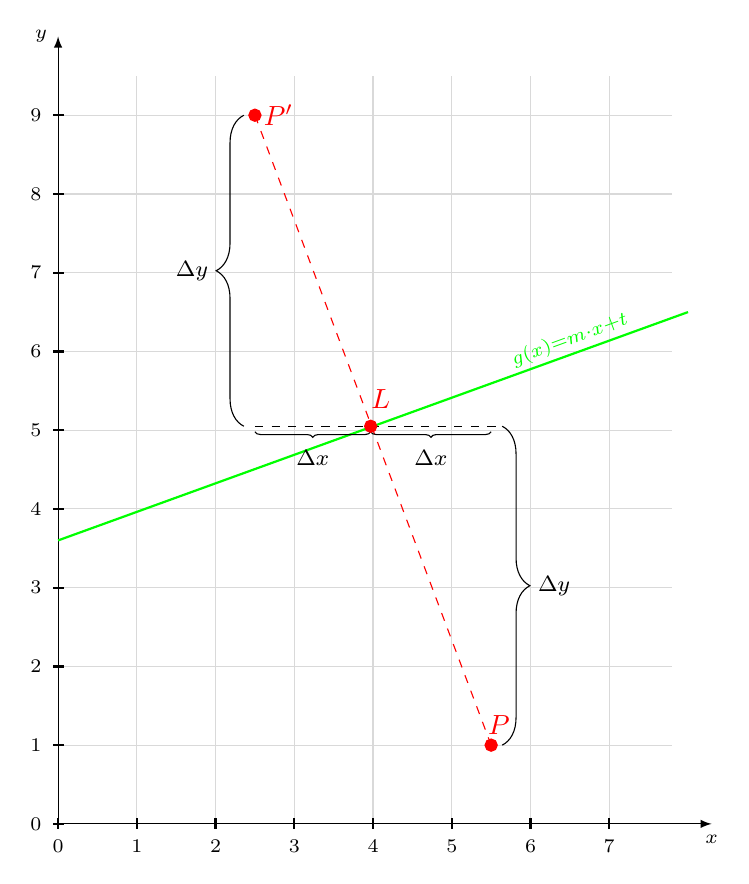
\begin{tikzpicture}
       \tkzInit [xmin=0,xmax=7.8,ymin=0,ymax=9.5]
        \begin{scriptsize}
            \tkzGrid[color = gray!30!white]
            \tkzAxeXY
        \end{scriptsize}
        \draw[thick,green] (0,3.6) -- (8,6.5);
        \node[green,rotate=20] at (6.5,6.15) {$\scriptstyle g(x) = m \cdot x + t$};

        \draw[dashed,red] (5.5,1) -- (2.5,9);

        \draw[thick,fill=red,red] (5.5,1) circle (2pt);
        \node[red] at (5.6,1.25) {$P$};

        \draw[thick,fill=red,red] (2.5,9) circle (2pt);
        \node[red] at (2.8,9) {$P'$};

        \draw[dashed] (2.5,5.05) -- (5.6,5.05);

        \draw [decorate,decoration={brace,amplitude=10pt,mirror,raise=4pt},yshift=0pt]
        (5.5,1) -- (5.5,5.05)  node [black,midway,xshift=0.8cm] {\footnotesize
        $\Delta y$};

        \draw [decorate,decoration={brace,amplitude=10pt,mirror,raise=4pt},yshift=0pt]
        (2.5,9) -- (2.5,5.05)  node [black,midway,xshift=-0.8cm] {\footnotesize
        $\Delta y$};

        \draw [decorate,decoration={brace,amplitude=2pt,mirror,raise=2pt},yshift=0pt]
        (2.5,5.05) -- (3.97,5.05)  node [black,midway,yshift=-0.4cm] {\footnotesize
        $\Delta x$};

        \draw [decorate,decoration={brace,amplitude=2pt,mirror,raise=2pt},yshift=0pt]
        (3.97,5.05) -- (5.5,5.05)  node [black,midway,yshift=-0.4cm] {\footnotesize
        $\Delta x$};

        \draw[thick,fill=red,red] (3.97,5.05) circle (2pt);
        \node[red] at (4.1,5.4) {$L$};
\end{tikzpicture}
\end{document}
